
\section{Validation case studies}\label{sec:validation} 

``Validation'' describes the comparison of numerical model output with physical observations in cases where the observations are sufficiently-complete and of sufficient quality so that the performance of the numerical model can be assessed \cite{Roache,Wesseling}.  Roughly speaking, validation can happen when the observations or data are better than the model, so the comparison measures the quality of the numerical model and not merely errors in, or incompleteness of, the data.  Because of the difficulty of measuring boundary conditions for real ice flows, this situation is not automatic in glaciology, or even common.\footnote{Which explains the rise of ``simplified geometry intercomparisons''; see section \ref{sec:simp}.}  Nonetheless we try two cases, first where PISM is applied on millimeter scale to model a laboratory experiment, and second for a large-scale ice flow in which all uncertainties of bedrock topography, basal sliding, and subglacial hydrology are removed, namely a present-day ice shelf.

\subsection{An SIA flow model for a table-top laboratory experiment}\label{sec:labgum}
\index{PISM!validation of SIA flow model} \index{validation!SIA flow model}

Though there are additional complexities to the flow of real ice sheets, an ice sheet is a shear-thinning fluid with a free surface.  PISM ought to be able to model such flows in some generality.  We test that ability here by comparing PISM's isothermal SIA numerical model to a laboratory observations of a 1\% Xanthan gum suspension in water in a table-top, moving-margin experiment by R.~Sayag and M.~Worster \cite{SayagWorster2013,SayagPeglerWorster2012}.  The ``gum'' fluid is more shear-thinning than ice, and it has much lower absolute viscosity values, but it has the same density.  This flow has total mass $\sim 1$ kg, compared to $\sim 10^{18}$ kg for the Greenland ice sheet.

We compare our numerical results to the ``constant-flux'' experiment from \cite{SayagWorster2013}.  To clarify the experimental setup, Figure \ref{fig:labgumexperiment} reproduces Figures 2(c) and 2(d) from that reference.  A pump pushes the translucent blue-dyed fluid through a round 8 mm hole in the middle of a flat, clear table at a mass rate of about 3 gm/s.  The downward-pointing camera, which produced the right-hand figure, allows measurement of the location of margin of the ``ice cap'', and in particular of its radius.  These measured radii data are the ``$\times$'' symbols in Figure \ref{fig:labgumresult}.

\begin{figure}[ht]
\centering
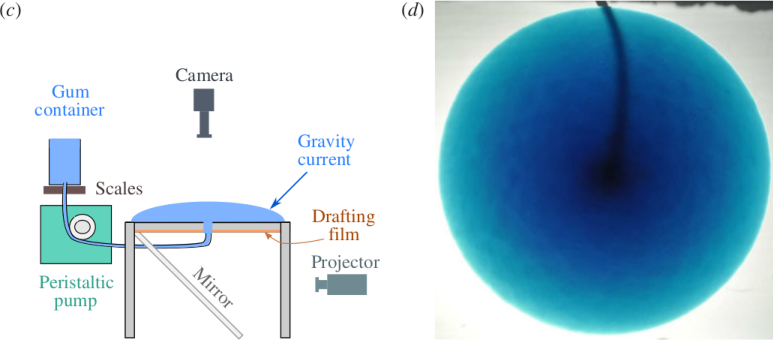
\includegraphics[width=6.0in,keepaspectratio=true]{labgumexperiment}
\caption{Reproduction of Figures 2(c) and 2(d) from \cite{SayagWorster2013}.  Left: experimental  apparatus used for ``constant-flux release'' experiment.  Right: snapshot of constant-flux experiment (plan view), showing an axisymmetric front.}
\label{fig:labgumexperiment}
\end{figure}

The closest glaciological analog would be an ice sheet on a flat bed fed by positive basal mass balance (i.e.~``refreeze'') underneath the dome, but with zero mass balance elsewhere on the lower and upper surfaces.  However, noting that the mass-continuity equation is vertically-integrated, we model the input flux (mass balance) as arriving at the \emph{top} of the ice sheet, as it is easier using PISM's climate input mechanisms.  The flow though the input hole is assumed to be constant across the hole, so the input ``climate'' has uses \texttt{-surface given} with a field \texttt{climatic_mass_balance}, in the bootstrapping file, which is a positive constant in the hole and zero outside.  While replacing flow into the base by mass balance at the top represents a very large change in the vertical component of the velocity field, we still see good agreement in the overall shape of the ``ice sheet'', and specifically in the rate of margin advance.

Sayag \& Worster estimate Glen exponent $n = 5.9$ for the flow law of their gum suspension, using regression of laboratory measurements of the radius.  Resetting this exponent is one of several changes to the configuration parameters, compared to PISM ice sheet defaults.  This is done in part by overriding parameters at run time by using the \texttt{-config_override} option.  See \texttt{examples/labgum/preprocess.py} for these settings.

To run the example, first do
\begin{verbatim}
$ python preprocess.py
\end{verbatim}
%$ - match dollar signs to make emacs happy
and then do a run for 746 model seconds \cite{SayagWorster2013} on an 10 mm grid (520 mm / 52 subintervals) using 4 processors:
\begin{verbatim}
$ ./rungum.sh 4 53 &> out.lab53 &
\end{verbatim}
%$ - match dollar signs to make emacs happy
This run generates text file \texttt{out.lab53}, diagnostic files \texttt{ts_lab53.nc} and \texttt{ex_lab53.nc}, and final output \texttt{lab53.nc}.  The run took about 5 minutes on a 2013 laptop; roughly real time!

When it is done, you can compare the modeled radius to the experimental data:
\begin{verbatim}
$ ./showradius.py -o r53.png -d constantflux3.txt ts_lab53.nc
\end{verbatim}
%$ - match dollar signs to make emacs happy
You can also redo the whole thing on a higher resolution grid (here: 2.5 mm), and when that run is done after several hours, make a combined figure just like Figure \ref{fig:labgumresult}:
\begin{verbatim}
$ ./preprocess.py -Mx 209 -o initlab209.nc
$ ./rungum.sh 4 209 &> out.lab209 &
$ ./showradius.py -o foo.png -d constantflux3.txt ts_lab*.nc
\end{verbatim}
%$ - match dollar signs to make emacs happy

\begin{figure}[ht]
\centering
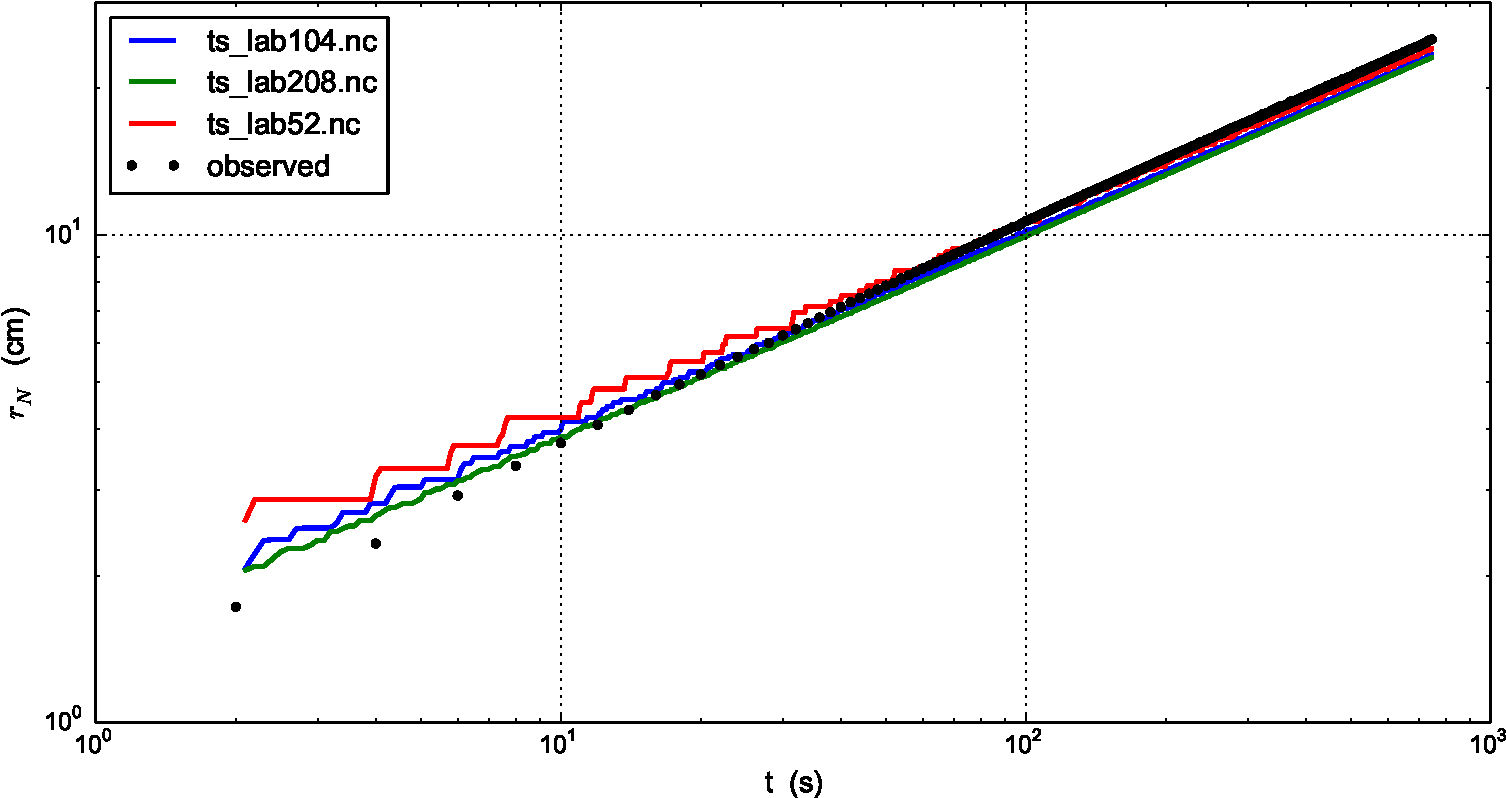
\includegraphics[width=6.0in,keepaspectratio=true]{labgumradius}
\caption{Radius $r_N(t)$ for runs with 10 mm (\texttt{ts_lab53.nc}) and 2.5 mm (\texttt{ts_lab209.nc}) grids, compared to observations from Sayag \& Worster's \cite{SayagWorster2013} table-top ``ice cap'' (gravity current) made from a 1 \% Xanthan gum suspension, as shown in Figure \ref{fig:labgumexperiment}.}
\label{fig:labgumresult}
\end{figure}

Results are better on finer grids, especially at small times, because the input hole has radius of only 8 mm.  Furthermore the ``ice cap'' has radius comparable to the hole for the first few model seconds.  Also the early evolution is distinctly non-shallow, but increasing resolution reduces most of the observations-simulation difference.  In fact, we know there is little need for ``higher-order'' stresses because the exact similarity solution of the shallow continuum equations, used by Sayag \& Worster, closely-fits the data even for small radius and time \cite[Figure 4]{SayagWorster2013}.  In any case, the large-time observations are closely-fit by the numerical results at all grid resolutions.


\subsection{An SSA flow model for the Ross Ice Shelf in Antarctica}\label{sec:ross} \index{PISM!diagnostic Ross ice shelf model}\index{Ice Sheets!Antarctic ice sheet!Ross ice shelf} \index{PISM!validation of SSA ice shelf model}\index{validation!SSA ice shelf model} \index{Ross ice shelf}
\optsection{Ross ice shelf}

As part of the EISMINT series of intercomparisons, MacAyeal and others \cite{MacAyealetal} successfully validated early-1990s ice shelf numerical models using velocity data for the Ross ice shelf.  The data were from the RIGGS survey \cite{RIGGS2}, acquired in the period 1973--1978 and measured at a few hundred locations in a grid across the shelf.  Substantial modelling developments followed EISMINT-Ross, including inverse modeling to recover depth-averaged viscosity \cite{RommelaereMacAyeal} and parameter-sensitivity studies \cite{HumbertGreveHutter}.  Previous PISM versions set up the EISMINT-Ross flow model and performed the diagnostic computation, with RIGGS data for validation.

However, availability of rich new data sets for ice sheet modeling, including the ALBMAP v1 \cite{LeBrocqetal2010} ice sheet geometry, bedrock, and climate data set, and the radar-derived (InSAR) MEaSUREs Antarctica Velocity Map \cite{Rignotetal2011}, allows us to use more complete, recent, and higher-resolution data for the same basic job.  Furthermore one can extend the diagnostic Ross ice shelf calculation both to other ice shelves around Antarctica and to time-evolving (``prognostic'') cases using the eigencalving \cite{Levermannetal2012} mechanisms.

The scripts in this subsection are found in directory \texttt{examples/ross/}.  In summary, the script \texttt{preprocess.py} downloads data and builds a NetCDF input file for PISM.  For the diagnostic computation we document first, the script \texttt{run_diag.sh} (in subdirectory \texttt{examples/ross/diagnostic/}) runs PISM.  The script \texttt{plot.py} shows a comparison of observations and model results, as in Figure \ref{fig:rosspython}.

\subsubsection*{Preprocessing the data}  The script \texttt{preprocess.py} downloads ALBMAP and MEaSUREs NetCDF files using \texttt{wget}; these files total around 100 Mb.  Then it uses NCO to cut out the relevant portion of the grid and CDO to conservatively-interpolate the high-resolution (500 m) velocity data onto the coarser (5 km) geometry grid used in ALBMAP.  The script \texttt{nc2cdo.py} from directory \texttt{util/}, prepares the NetCDF file for the application of CDO, which requires complete projection information.  Do

\begin{verbatim}
$ cd examples/ross/
$ ./preprocess.py
\end{verbatim}
%$ - match dollar signs to make emacs happy

The NetCDF file \texttt{Ross_combined.nc} produced by \texttt{preprocess.py} contains ice thickness, bed elevations, surface temperature, net accumulation, as well as latitude and longitude values.  All of these are typical of ice sheet modelling data, both in diagnostic runs and as needed to initialize and provide boundary conditions for prognostic (evolutionary) runs; see below for the prognostic case with these data.  The \texttt{_combined} file also has variables \texttt{u_ssa_bc} and \texttt{v_ssa_bc} for the boundary values used in the (diagnostic and prognostic) computation of velocity.  They are used at all grounded locations and at ice shelf cells that are immediate neighbors of grounded ice.  The variable \texttt{bc_mask} specifies these locations.  Finally the variables \texttt{u_ssa_bc,v_ssa_bc}, which contain observed values, are used after the run to compare to the computed interior velocities.

\subsubsection*{Diagnostic computation of ice shelf velocity}  The diagnostic velocity computation bootstraps from \texttt{Ross_combined.nc} and does a zero-year run; in the $211\times 211$ grid case we demonstrate below, the key parts of the PISM command are

\begin{verbatim}
pismr -boot_file ../Ross_combined.nc -Mx 211 -My 211 -Mz 3 -Lz 3000 -z_spacing equal \
    -surface given -stress_balance ssa -energy none -yield_stress constant -tauc 1e6 \
    -pik -ssa_dirichlet_bc -y 0 -ssa_e 0.6 -ssafd_ksp_monitor
\end{verbatim}
%$ - match dollar signs to make emacs happy

\noindent The computational grid here is the ``native'' $5$ km data grid used in ALBMAP.  Regarding the options,

\begin{itemize}
\item The maximum thickness of the ice is $2766$ m so we choose a height for the computational box large enough to contain the ice (i.e.~\texttt{-Lz 3000}).  Vertical grid resolution is, however, unimportant in this case because we use the SSA stress balance only, and the temperature set at bootstrapping suffices to determine the ice softness; thus the options \texttt{-Mz 3 -z_spacing equal -energy none}.

\item Option \texttt{-stress_balance ssa} selects the SSA stress balance and turns off the SIA stress balance computation, since our goal is to model the ice shelf.  It also side-steps a technical issue: PISM uses periodic boundary conditions at domain boundaries and most fields in this setup are not periodic.  Turning off SIA avoids operations such as differencing surface elevation across the domain edges.  For a more complete solution to this technical issue see section \ref{sec:jako} about a regional model using option \verb|-no_model_strip| and executable \verb|pismo|.

\item Option \texttt{-y 0} chooses a diagnostic run.

\item Option \texttt{-pik} is equivalent to \texttt{-cfbc -kill_icebergs} in this non-evolving example.  Note that \texttt{-kill_icebergs} removes effectively-detached bits of ice, especially in McMurdo sound area, so that the SSA problem is well-posed for the grounded-ice-sheet-connected ice shelf.

\item Option \intextoption{ssa_dirichlet_bc} forces the use of fields \texttt{u_ssa_bc,v_ssa_bc,bc_mask} described above.  The field \texttt{bc_mask} is $1$ at boundary condition locations, and $0$ elsewhere.  For the prognostic runs below, the ice thickness is also fixed at boundary condition locations, so as to prescribe ice flux as an ice shelf input.

\item Options \texttt{-yield_stress constant -tauc 1e6} essentially just turn off the grounded-ice evolving yield stress mechanism, which is inactive anyway, and force a high resistance under grounded ice so it does not slide.  

\item Option \texttt{-ssa_e 0.6} is the single tuned parameter; this value gives good correlation between observed and modeled velocity magnitudes.

\item Option \texttt{-ssafd_ksp_monitor} provides feedback on the linear solver iterations ``underneath'' the nonlinear (shear-thinning) SSA solver iteration.
\end{itemize}

There is no need to type in the above command; just do

\begin{verbatim}
$ cd diagnostic/
$ ./run_diag.sh 2 211 0.6
\end{verbatim}
%$ - match dollar signs to make emacs happy

Note \texttt{run_diag.sh} accepts three arguments: \texttt{run_diag.sh N Mx E} does a run with
\texttt{N} MPI processes, an \texttt{Mx} by \texttt{Mx} grid, and option \texttt{-ssa_e E}.  The choices above give a run which only takes a few seconds, and it produces output file \texttt{diag_Mx211.nc}.

There are many reasonable choices for the effective softness of an ice shelf, as ice density, temperature, and the presence of fractures all influence the effective softness.  Using an enhancement factor \texttt{-ssa_e 0.6} acknowledges that the physical justification for tuning the ice softness is uncertain.  One could instead use the temperature itself or the ice density\footnote{High accumulation rates, cold firn with minimal compression, and basal freeze-on of marine ice may all generate significant variation in shelf density.} as tuning parameters, and these are worthwhile experiments for the interested PISM user.

The script \texttt{plot.py} takes PISM output such as \texttt{diag_Mx211.nc} to produce Figure \ref{fig:rosspython}.  The run shown in the figure used an enhancement factor of $0.6$ as above.  The thin black line outlines the floating shelf, which is the actual modeling domain here.  To generate this Figure yourself, do

\begin{verbatim}
$ ../plot.py diag_Mx211.nc
\end{verbatim}
%$ - match dollar signs to make emacs happy

\begin{figure}[ht]
\centering
\mbox{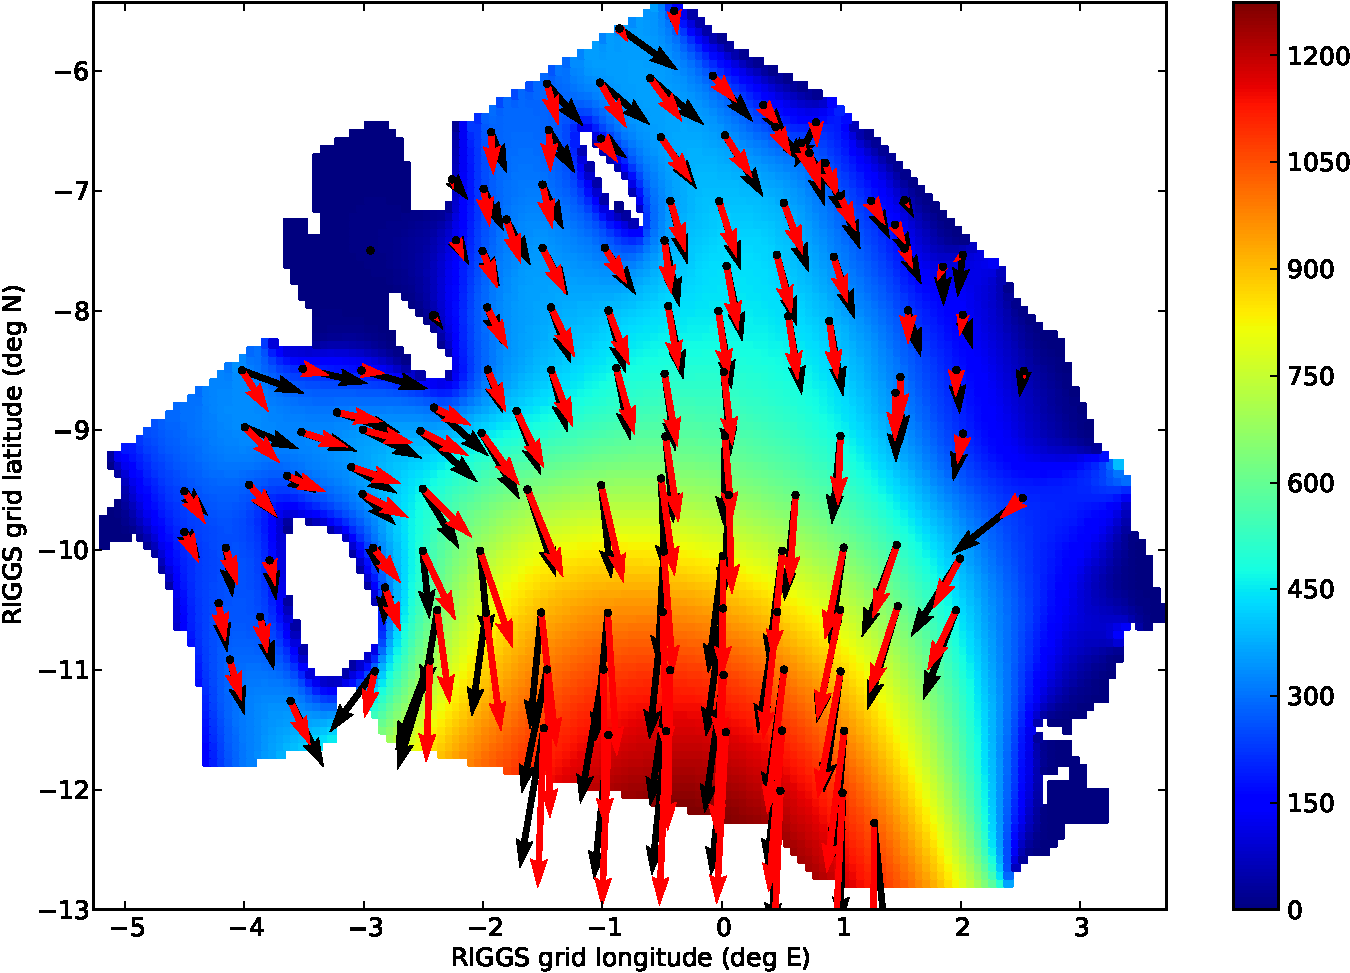
\includegraphics[width=3.3in,keepaspectratio=true]{rossquiver}\quad 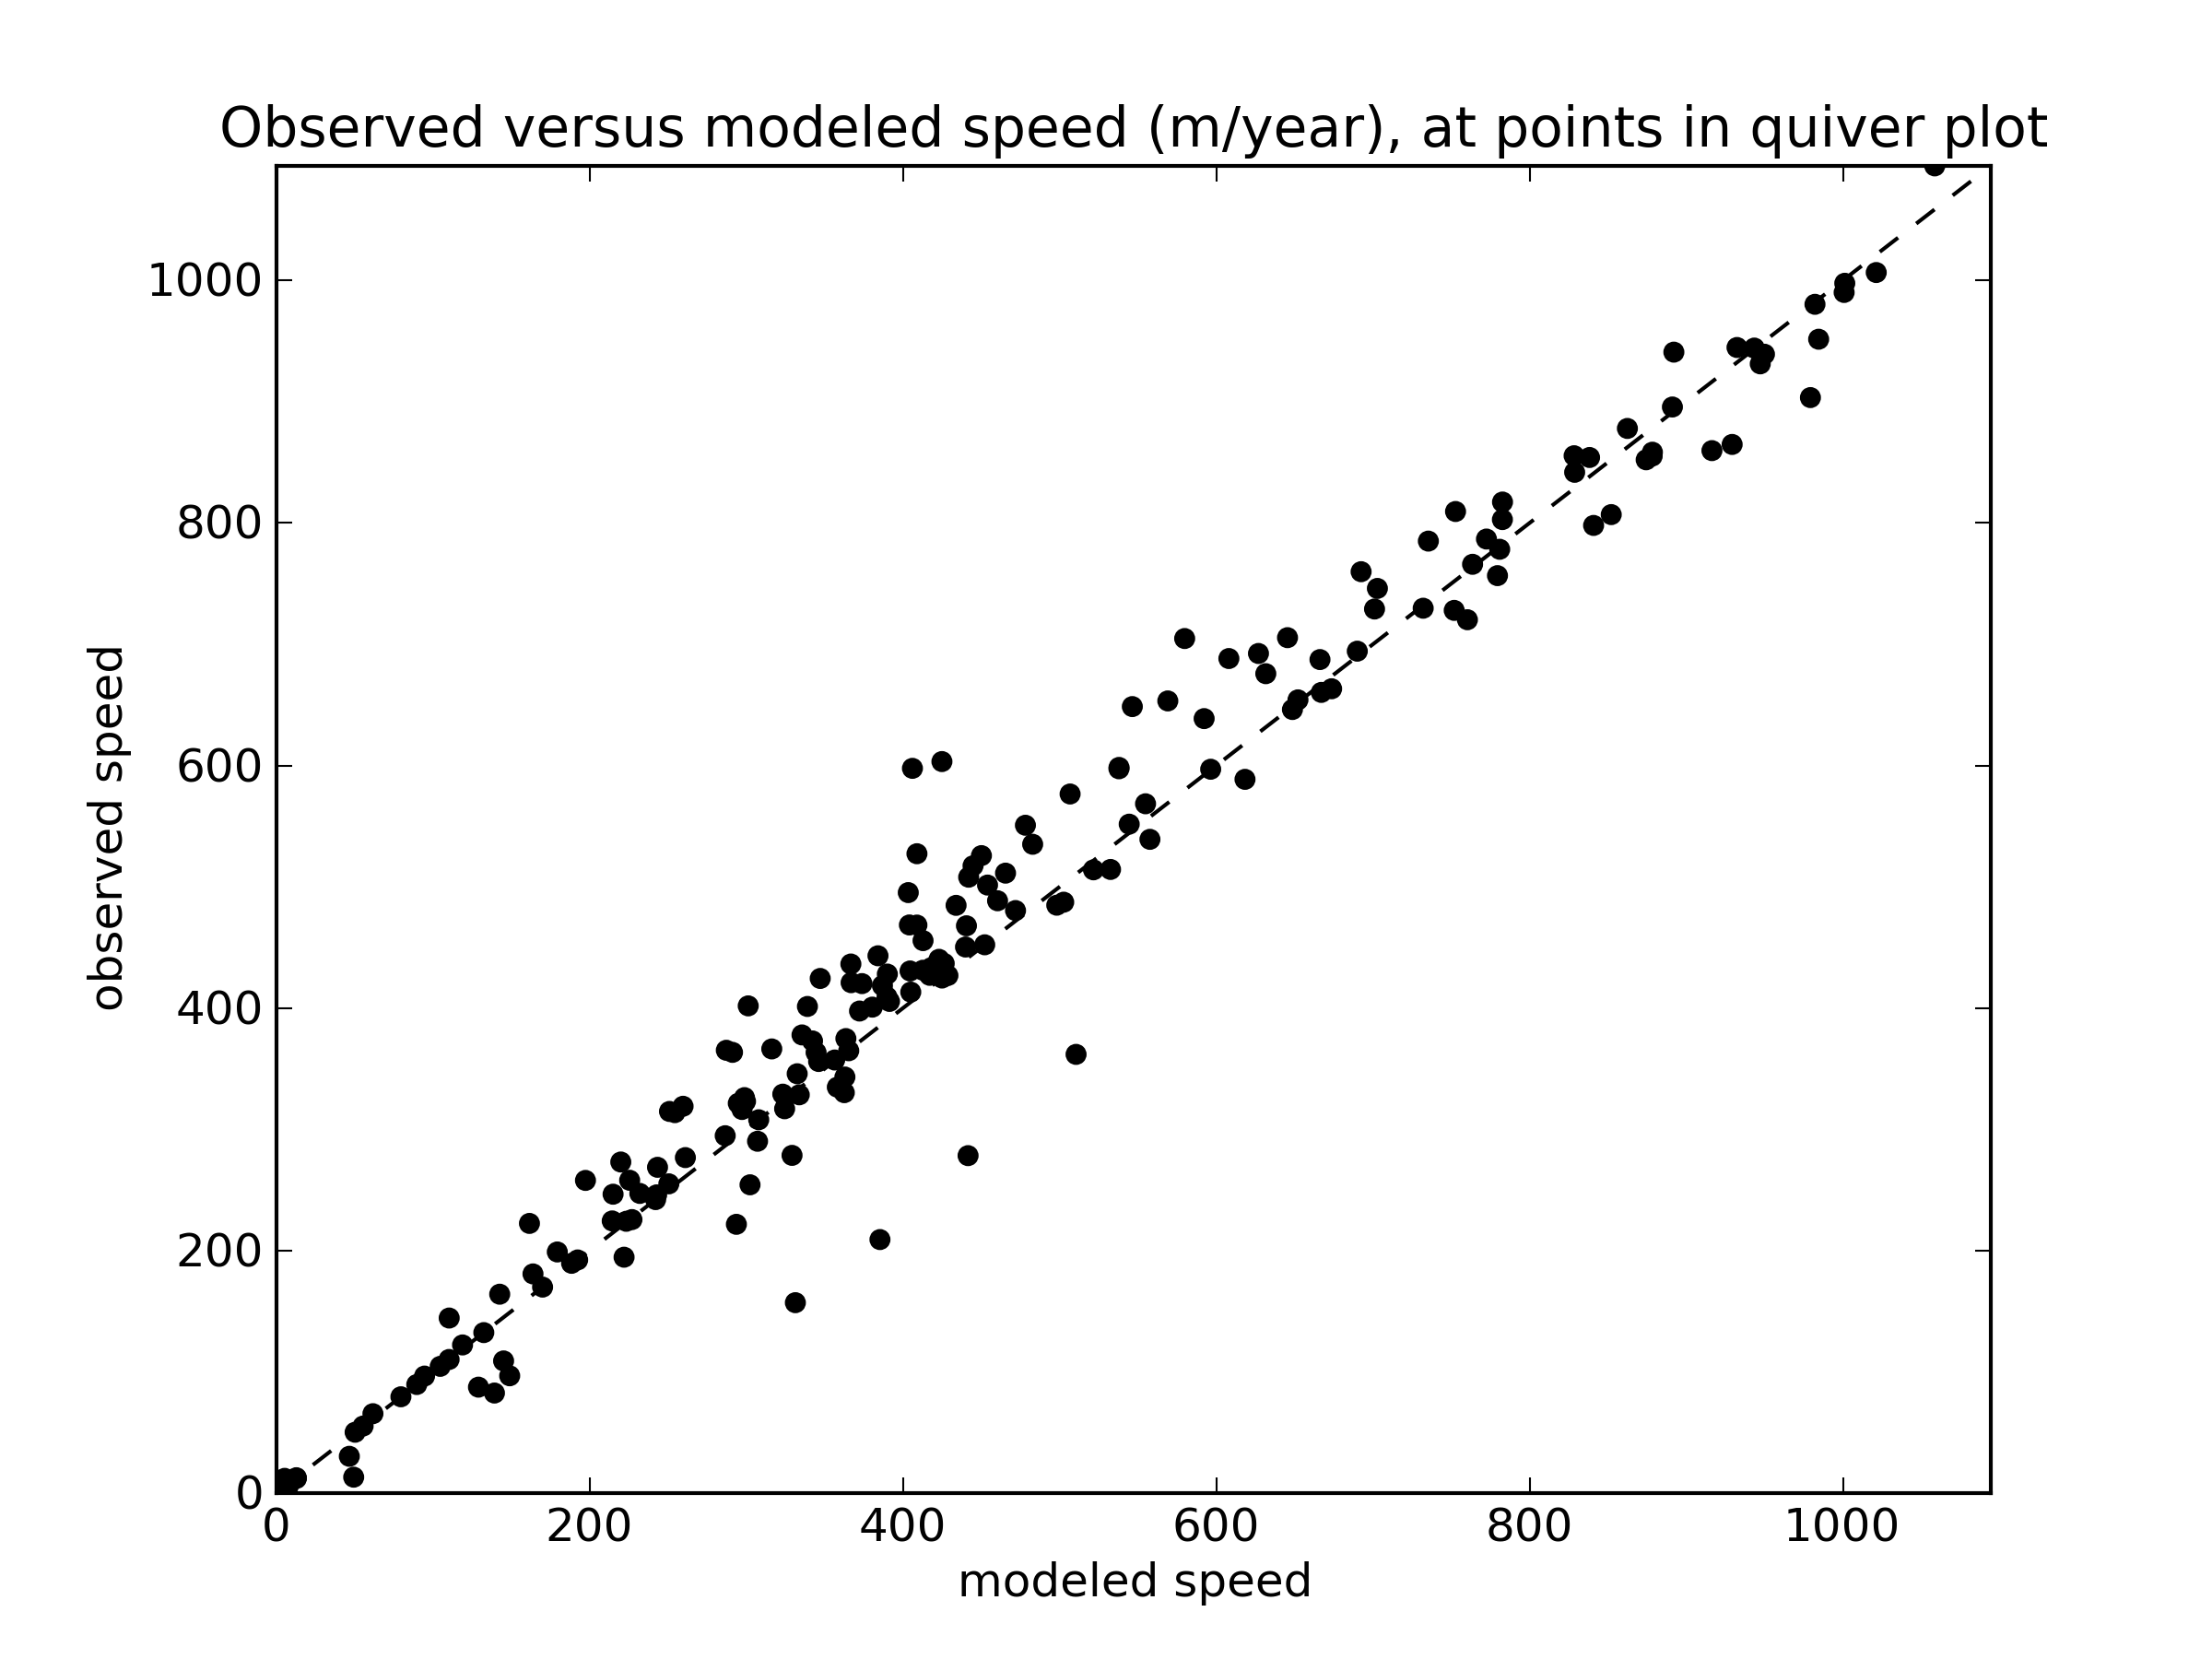
\includegraphics[width=2.7in,keepaspectratio=true]{rossscatter}}
\caption{\protect{\emph{Left}}: Color is speed in m/a.  Arrows are observed (white) and modeled (black) velocities.  \protect{\emph{Right}}: Comparison between modeled and observed speeds at points plotted on the left.}
\label{fig:rosspython}
\end{figure}

\subsubsection*{Extending this example to other ice shelves}  The SSA diagnostic solution described in this section can be easily applied to other ice shelves in Antarctica, such as the Filchner-Ronne Ice Shelf modeled using PISM in \cite{AlbrechtLevermann2012}, for example.

Simply choose a different rectangular domain, within the area covered by the whole-Antarctic data-sets used here, at the preprocessing stage.  In particular you should modify the lines ``\texttt{ncks -O -d x1,439,649 -d y1,250,460 ...}'' (for ALBMAP data) and ``\texttt{ncks -d x,2200,3700 -d y,3500,4700 ...}'' (for MEaSUREs velocity data) in the script \texttt{examples/ross/preprocess.py}.

\subsubsection*{Prognostic modelling using eigencalving}  Next we summarize how you can create an evolving-geometry model of the Ross ice shelf with constant-in-time inflow across the fixed grounding line.  See \texttt{README.md} and \texttt{run_prog.sh} in \texttt{examples/ross/prognostic/}.  This example also demonstrates the \intextoption{calving eigen_calving} model for a moving calving front \cite{Levermannetal2012}.

Start by running \texttt{preprocess.py} in \texttt{examples/ross/} as described above.  If you have already done the diagnostic example above, then this stage is complete.

Then change to the \texttt{prognostic/} directory and run the default example:

\begin{verbatim}
$ cd examples/ross/prognostic/
$ ./run_prog.sh 4 211 0.6 100
\end{verbatim}
%$ - match dollar signs to make emacs happy    

\noindent This 100 model year run on 4 processes and a 5 km grid took about twenty minutes on a 2013 laptop.  It starts with a bootstrapping stage which does a \texttt{y 0} run, which generates \texttt{startfile_Mx211.nc}.  It then re-initializes to start the prognostic run itself.  See the \texttt{README.md} for a bit more on the arguments taken by \texttt{run_prog.sh} and on viewing the output files.

The PISM command done here is (essentially, and without showing diagnostic output choices)

\begin{verbatim}
pismr -i startfile_Mx211.nc -surface given -stress_balance ssa \
    -yield_stress constant -tauc 1e6 -pik -ssa_dirichlet_bc -ssa_e 0.6 \
    -y 100 -o prog_Mx211_yr100.nc -o_order zyx -o_size big \
    -calving eigen_calving,thickness_calving -eigen_calving_K 1e17 \
    -cfl_eigen_calving -thickness_calving_threshold 150.0 \
    -ssafd_ksp_type gmres -ssafd_ksp_norm_type unpreconditioned \
    -ssafd_ksp_pc_side right -ssafd_pc_type asm -ssafd_sub_pc_type lu
\end{verbatim}
%$ - match dollar signs to make emacs happy    

Several of these options are different from those used in the diagnostic case.  First, while the command \texttt{-pik} is the same as before, now each part of its expansion, namely \texttt{-cfbc -kill_icebergs -part_grid -part_redist}, is important.  As the calving front evolves (i.e.~regardless of the calving law choices), option \texttt{-part_grid} moves the calving front by one grid cell only when the cell is full of the ice flowing into it; see \cite{Albrechtetal2011}.  The option \texttt{-kill_icebergs} is essential to maintain well-posedness of the SSA velocity problem at each time step \cite{Winkelmannetal2011}.  See section \ref{sec:pism-pik}.

Option combination
\begin{verbatim}
    -calving eigen_calving,thickness_calving -eigen_calving_K 1e17 \
    -cfl_eigen_calving -thickness_calving_threshold 150.0
\end{verbatim}
%$ - match dollar signs to make emacs happy
specifies that ice at the calving front will be removed if either a criterion on the product of principal stresses is satisfied \cite{Levermannetal2012}, namely \texttt{eigen_calving} with the given constant $K$, or if the ice thickness goes below the given threshold of 150 meters.  See subsection \ref{sec:calving}.

There is also an extended option combination
\begin{verbatim}
    -ssafd_ksp_type gmres -ssafd_ksp_norm_type unpreconditioned \
    -ssafd_ksp_pc_side right -ssafd_pc_type asm -ssafd_sub_pc_type lu
\end{verbatim}
%$ - match dollar signs to make emacs happy
which tells the PETSc KSP object used by the SSA solver to solve in the most robust, though not necessarily fastest, way.  In particular, the linear problem is spread across processors using an additive Schwarz domain decomposition preconditioning method (\texttt{pc_type asm}) \cite{Smithetal1996}, along with the standard \texttt{gmres} KSP solver, and then on each processor the local part of the linear system is solved by a direct method by the preconditioner (\texttt{sub_pc_type lu}).  These choices seem to be effective for solving SSA stress balances on the complicated-geometry domains which arise from nontrivial calving laws.

%FIXME \textbf{Evolving fracture density.}  See \texttt{README.md}, \texttt{preprocess_frac.py}, and \texttt{run_frac.sh} in directory \texttt{examples/ross/fracture_density/}.  This example demonstrates the fracture density transport model in \cite{AlbrechtLevermann2012}.


%%% Local Variables:
%%% mode: latex
%%% TeX-master: "manual"
%%% End:
